\chapter{Personendetektion}
\label{chap:Personendetektion}

Auf der Grundlage der vorherigen Kapitel wird nun mittels einem neuronalen Netzwerk eine Personenerkennung erstellt. Dieser Abschnitt beschreibt das Vorgehen, um die Anzahl Personen in einem Aufzug zu erkennen. In einem ersten Schritt wird die Verarbeitung der Rohdaten aufgezeigt. Für den Auswertealgorithmus wurden mehrere unterschiedliche Aufzüge evaluiert und für jeden Aufzug ein Profil erstellt. 



\begin{figure}[H]
	\centering
	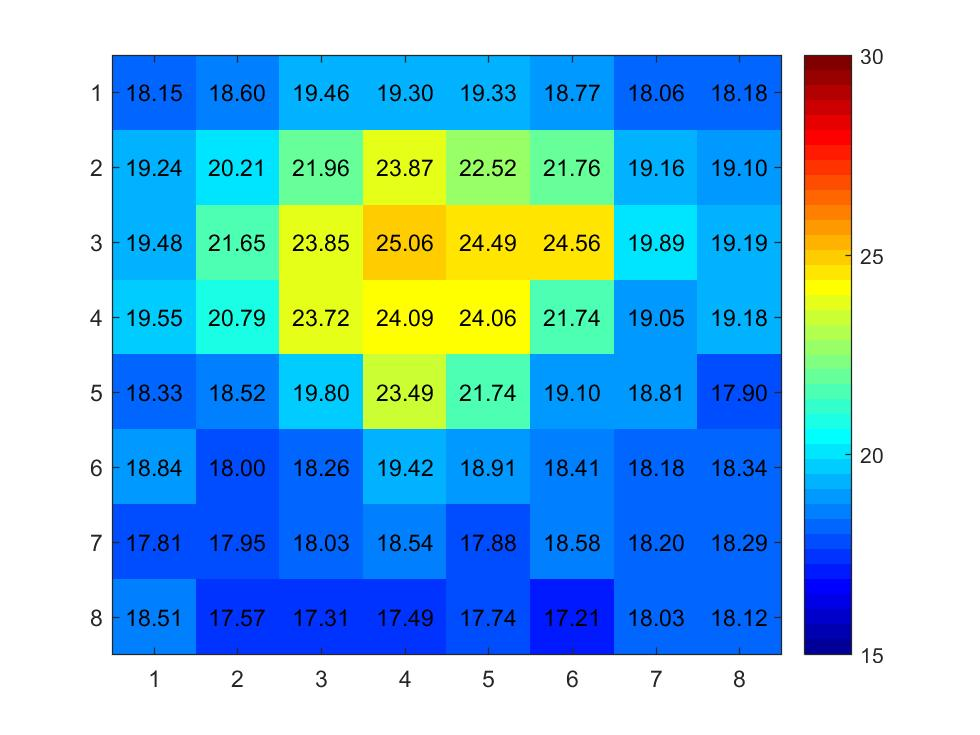
\includegraphics[width=0.5\textwidth]
	{fig/person_175_shirt.jpg}
	\caption[Pixeldarstellung einer Person]{Pixeldarstellung einer Person}
	\label{fig:Pixelbild}
\end{figure}



\section{Datenverarbeitung}




\section{Datenmanipulation mittels Interpolation}

Die Auflösung von 8x8 Pixel bietet nur begrenzte Aussagekraft über die Anzahl Personen in einem Aufzug. Daher wurde mittels MATLAB mehrere Interpolationsverfahren benutzt, um die Auflösung der Personenerkennung zu verbessern. Im Zusammenhang mit den Pixelwerten eignet sich bikubische und 



Da im Zusammenhang mit dem Auswertealgorithmus mittels TensorFlow





\section{Symmetrische Erweiterung}

Um die Datensätze zu vergrößern wurden die drei Profile erweitert. Dafür wurde für die entsprechenden Profile Python-Programm rotate\_and\_swap\_ProfilX  geschrieben, welche alle Frames er Datensätze symmetrisch erweitert.  

\begin{figure}[!ht]
	\centering
	\begin{minipage}[c]{0.35\linewidth}
	\centering
	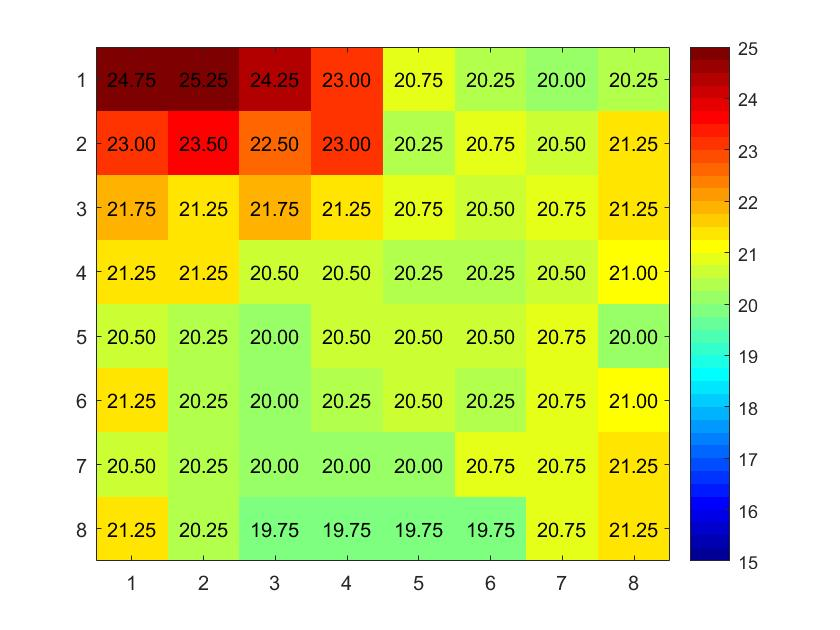
\includegraphics[width=.8\linewidth]{fig/original}
	\caption{Originales Frame}
	\label{fig:original}
	\end{minipage}
	\hfill
	\begin{minipage}[c]{0.6\linewidth  }
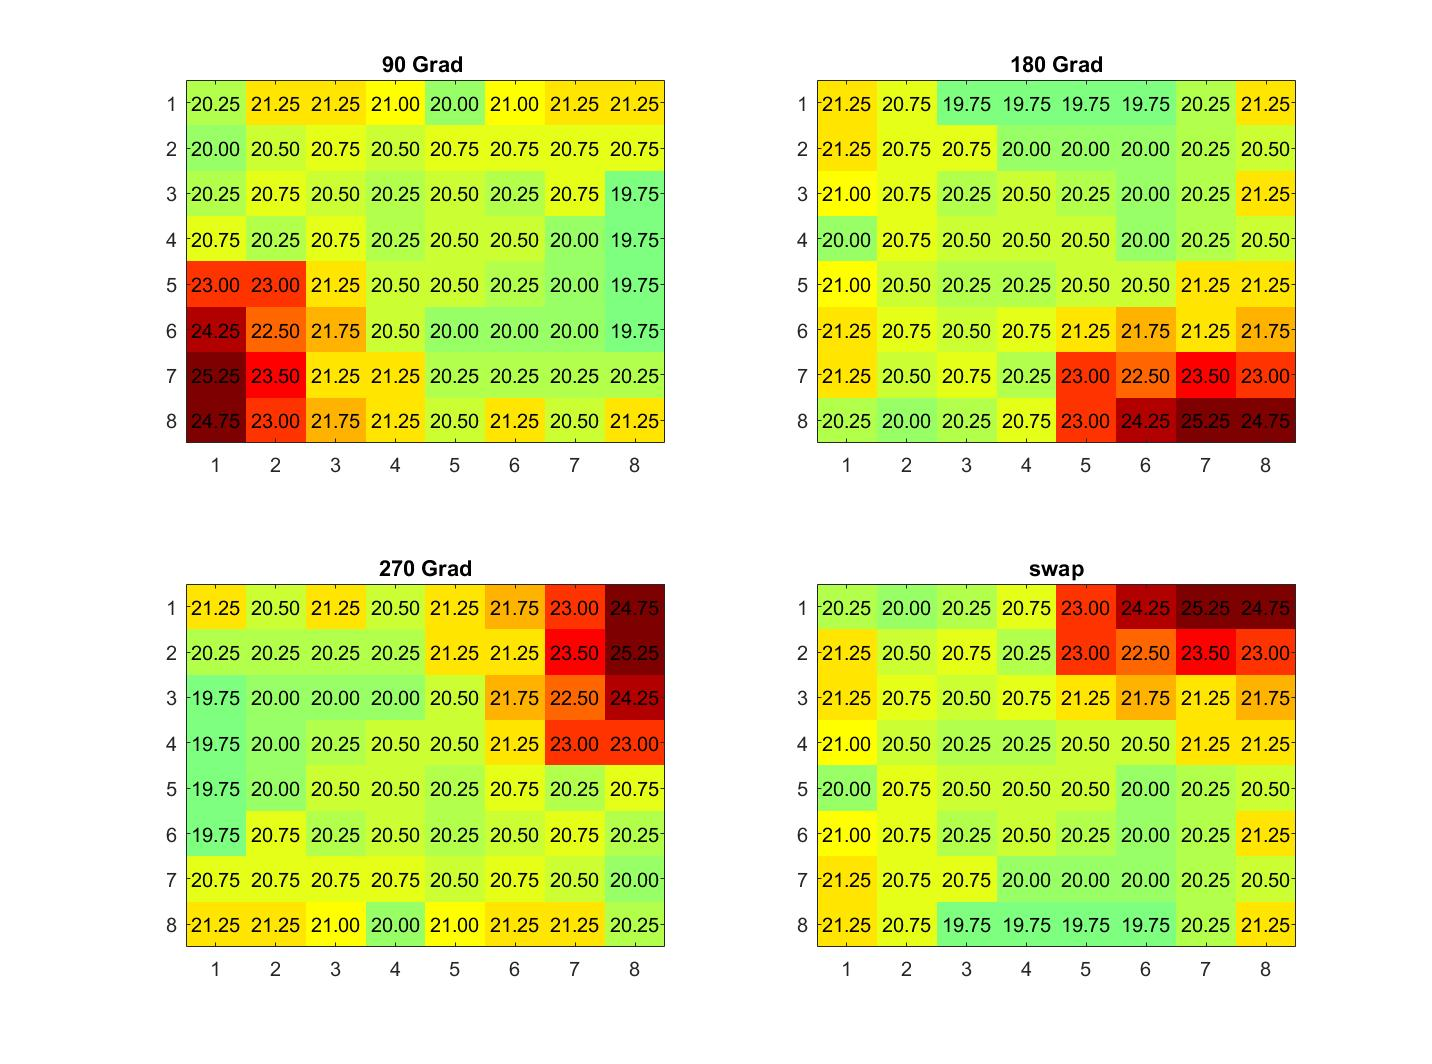
\includegraphics[width=1\linewidth]{fig/rotated}
\caption{Rotierte und gespiegelte Frames}
\label{fig:rotated}
	\end{minipage}
\end{figure}


Durch die Erweiterung konnten die Datensätze um den Faktor 5 vergrößert werden. Es konnten so, nicht vermessenen Positionen generiert werden. Mit den Messstandorten A-I und den generierten Erweiterungen werden nahezu beliebige Varianten im Messbereich zur Verfügung.


\subsection{Profilbildung}




Profil 1
Size of:
- Training-set:         126936
- Validation-set:       25000

Profil 2



Profil 3


Testprofil Test-set:             22169




\section{Aufbau Convolution Neural Network}




Convolutional Networks work by moving small filters across the input image. This means the filters are re-used for recognizing patterns throughout the entire input image. This makes the Convolutional Networks much more powerful than Fully-Connected networks with the same number of variables. This in turn makes the Convolutional Networks faster to train




The convolutional filters are initially chosen at random, so the classification is done randomly. The error between the predicted and true class of the input image is measured as the so-called cross-entropy. The optimizer then automatically propagates this error back through the Convolutional Network using the chain-rule of differentiation and updates the filter-weights so as to improve the classification error. This is done iteratively thousands of times until the classification error is sufficiently low.


(W -F +2P) : S+ 1



\begin{figure}[H]
	\centering
	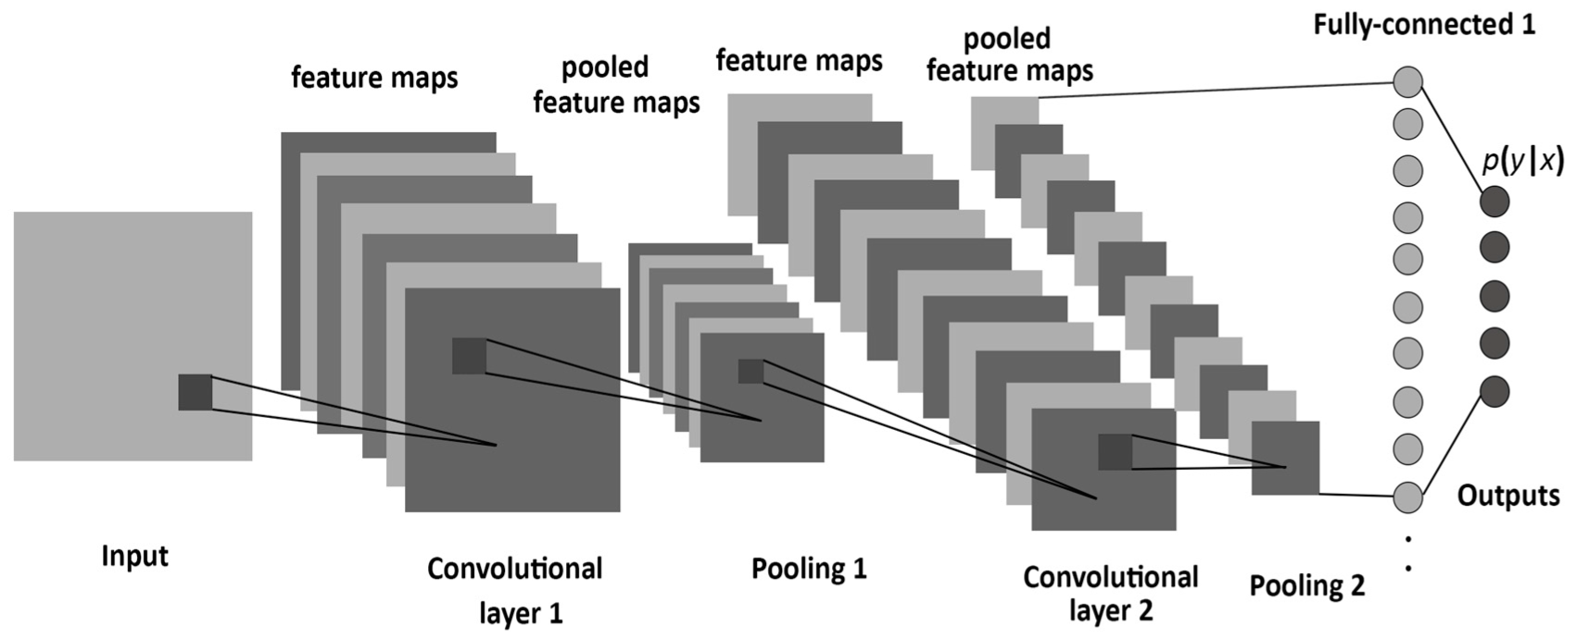
\includegraphics[width=1\textwidth]
	{fig/CCN.png}
	\caption[Aufbau des Convolutional Neural Network]{Aufbau des Convolutional Neural Network}
	\label{fig:CCN}
\end{figure}




\section{Training und Validierung}




\begin{figure}[H]
	\centering
	\caption{Trainingsverlauf Profil 1}
	\label{fig:traininsverlauf}
	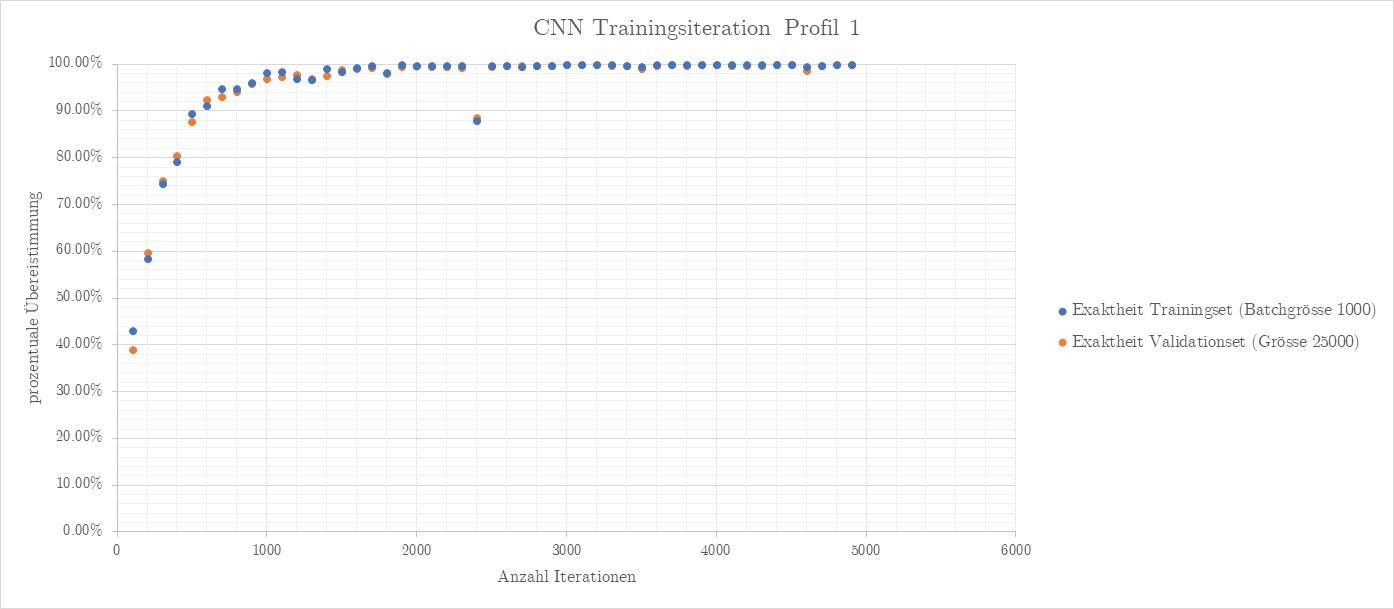
\includegraphics[width=1.0\linewidth]{fig/Traininsverlauf}
\end{figure}


\section{Ergebnisse}


\subsection{Profil 1}


\subsection{Profil 2}


\subsection{Profil 3}


\section{Echtzeitpersonenerkennung}

Dank der Saver-Klasse von Tensorflow lassen sich erstellte CNN-Modell als ckpt-File speichern. Dabei werden alle trainierten Bias und Gewichtungen in ein ckpt-File gespeichert. Diese lassen sich wiederum in ein untrainiertes CNN laden.

Auf dieser Grundlage wurde eine Messeinheit erstellt, welche mittels trainiertenn CNN zur Echtzeit Personerkennungen durchführt. Die Messeinheit besteht aus einenm AMG8834 Eval Kit, einem Raspbery Pi3 und einer Powerbank.

In Abbildung ist das 


\begin{figure}[H]
	\centering
	\caption{Trainingsverlauf Profil 1}
	\label{fig:Echtzeitmesseinheit}
	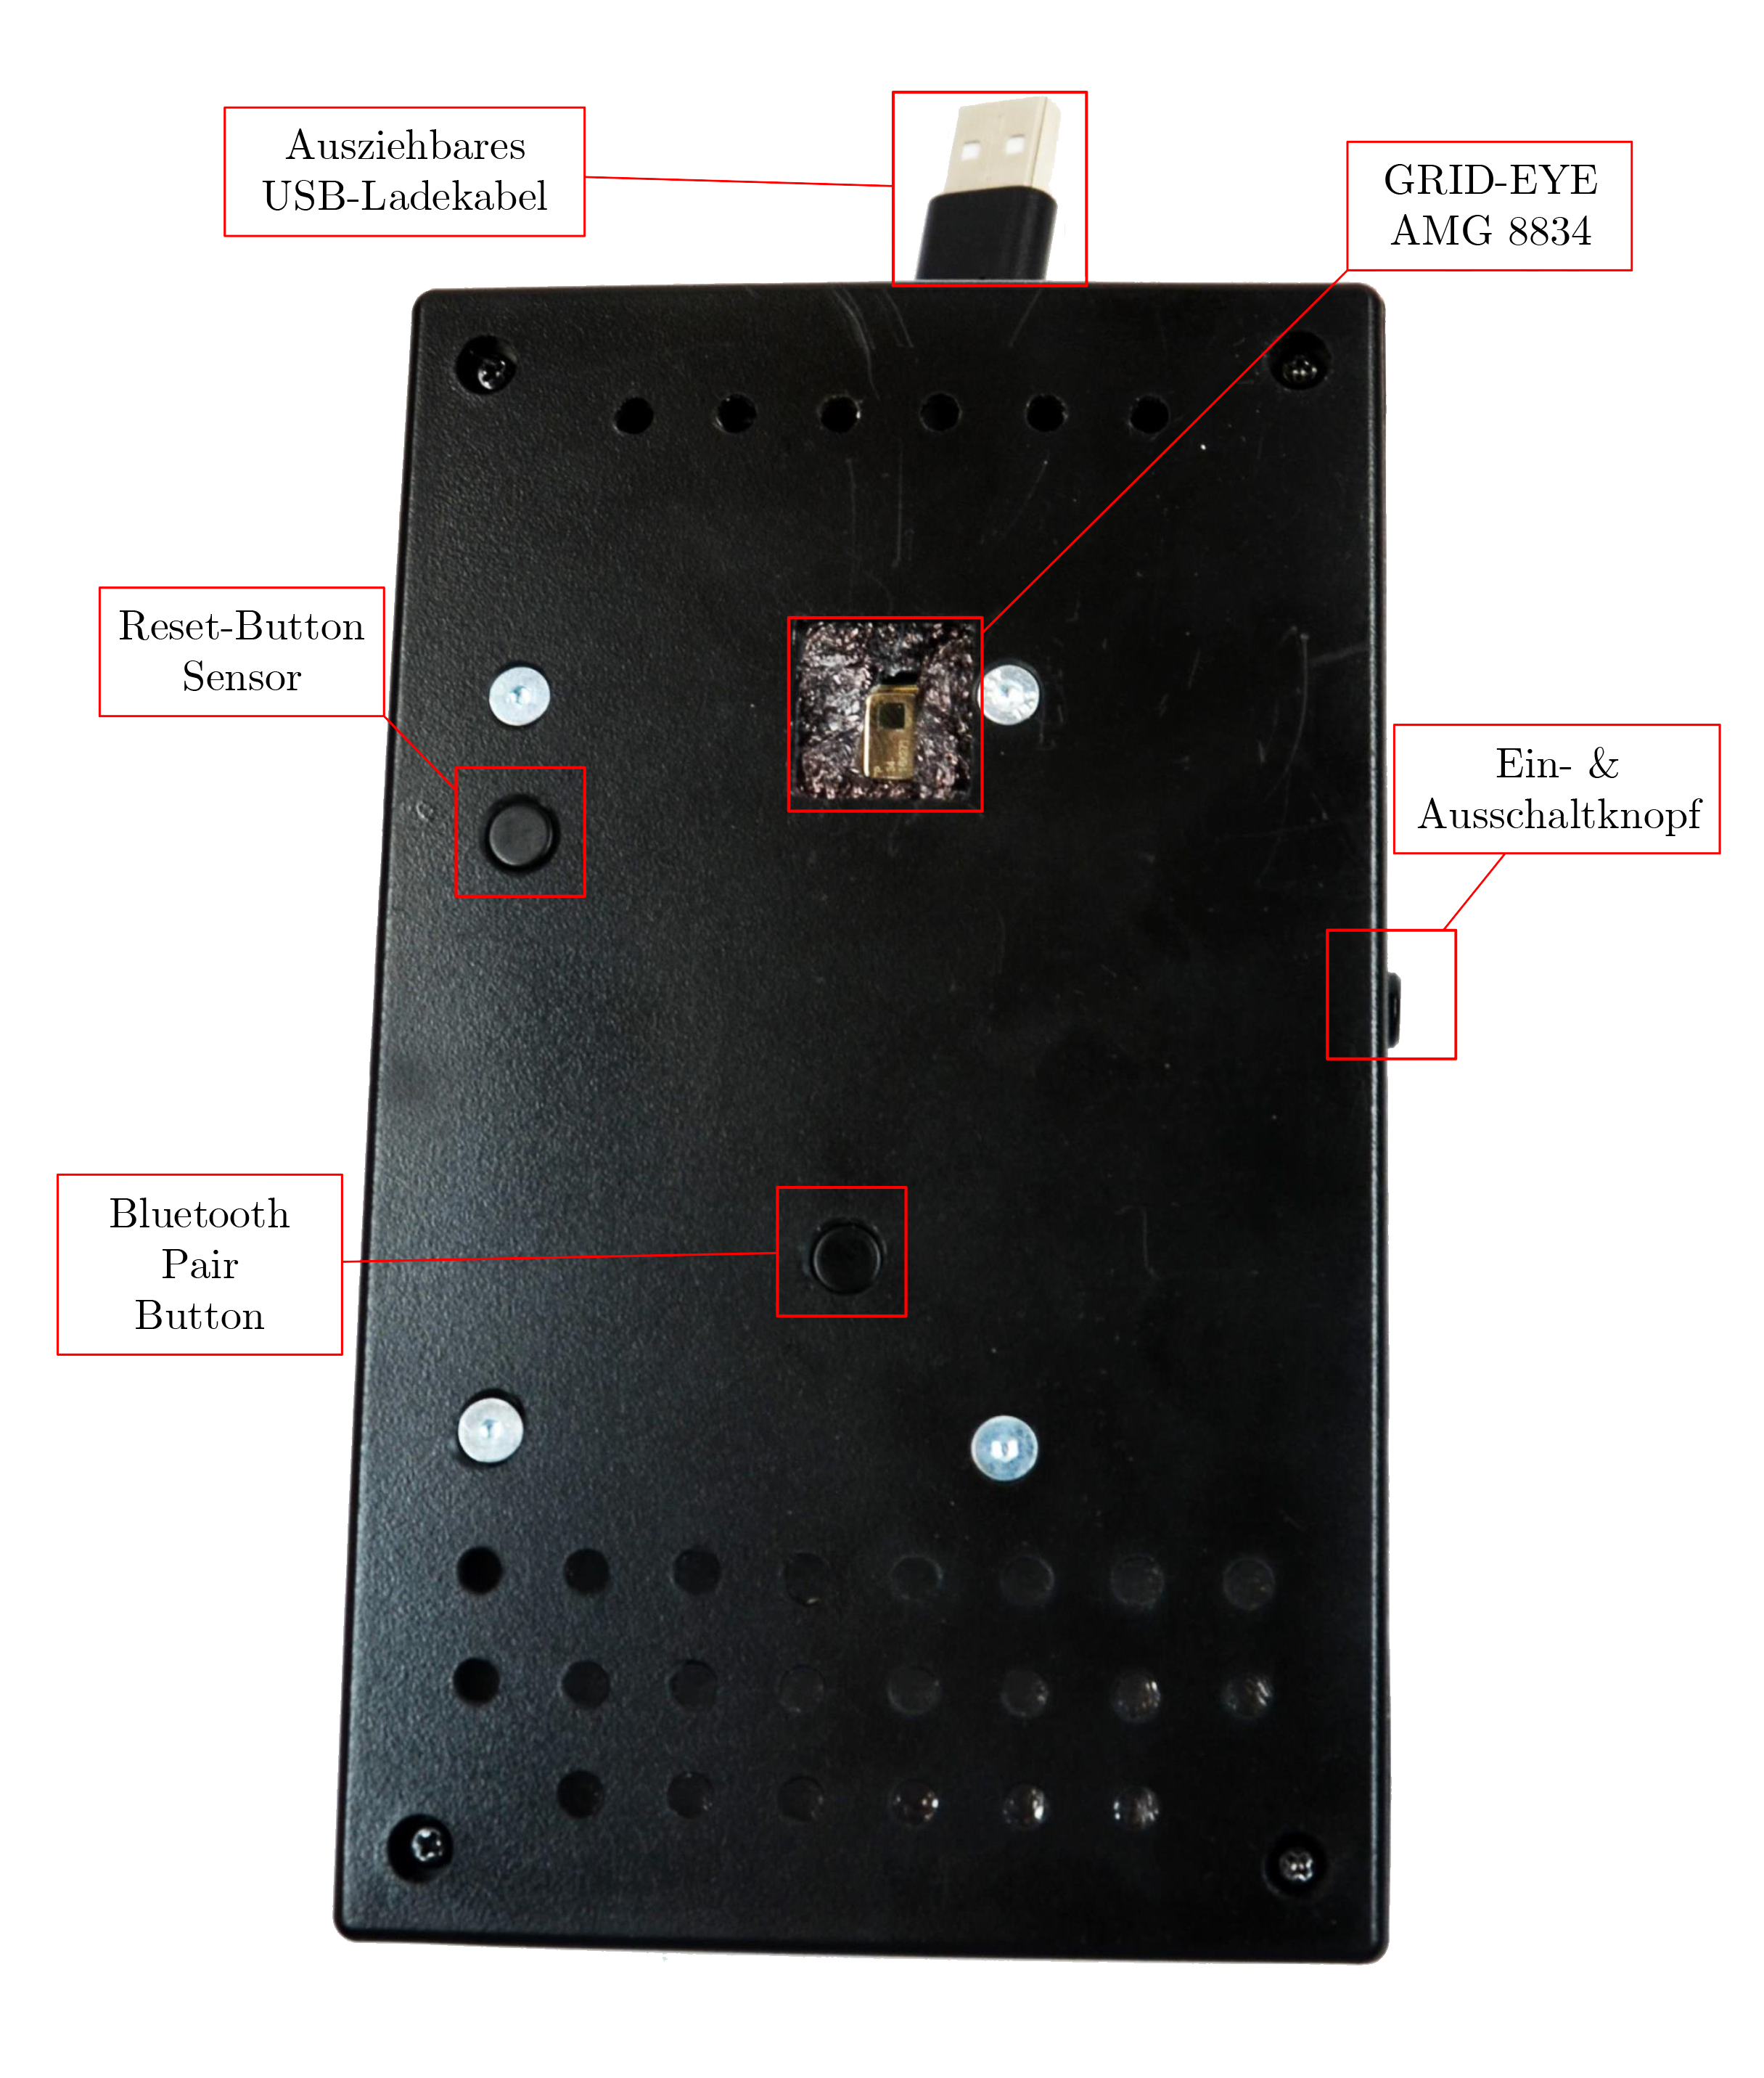
\includegraphics[width=1.0\linewidth]{fig/Echtzeitmessgeraet.jpg}
\end{figure}




\section{Fazit}

Tensorflow bietet mit der Implentierung \ac{CNN} eine grosse Anzahl an Parameter und varrierbaren Einstellungen, um eine Bilderkennung mittels maschinellen Lernens zu realiiseren. 

Der relevanteste Punkt für die Personenerkennung sind die Trainingssets. Es wurde mit den erstellten Datensätzen eine möglichst breite Platte an Situationen generiert, trotzdem lassen sich zum Teil Frames nicht differenzieren. Dies hat eines der folgenden Gründe.

Die Auflösung ist jedoch in diesem Zusammenhang. Da nur 8x8 Pixel zur Verfügung stehen, ist die Tiefe de neuronalen Netzwerk begrenzt. Es lassen sich viele Features aus den Frames generieren , doch die Unterschiede zu anderen Objekten lassen sich nur bedingt erstellen.

Die Genauigkeit des Sensors streut mit 3°C bedeutend. Dies verursacht das die bedeutend mehr unterschiedliche thermische Frames vorhanden sind, doch die Streuung verursacht eine grösse Messunsicherheit, welche vorallem bei Bilder zu tragen kommen, in welchen mehrere Personen von unterschieldicher Grösse nahe beinader stehen. Durch die Unsicherheit lassen sich einzelne grosse Personen kaum von mehreren kleinen Personen differenzieren.






